% Thesis introduction
% Author: Tore.
%

In this chapter the background information needed in order to understand the topics of this thesis and its papers is given. First, in Section \ref{sec:gpgpu}, general-purpose programming on graphics processing units (\nom{GPGPU}{General-purpose programming on graphics processing units}) is reviewed, followed by an introduction to medical ultrasound imaging in Section \ref{sec:ultrasound}. Finally, the concepts of volume rendering and ultrasound field simulations are presented in Section \ref{sec:volren} and \ref{sec:field}.

\section{General-purpose computing on graphics processing units}\label{sec:gpgpu}
In a recent essay, Herb Sutter, a leading authority on software development, reviews the current state of the software and computer industry \cite{HerbSutter}. The essay bears the name "Welcome to the Jungle" and is a sequel to the essay "The Free Lunch is Over" from 2004 \cite{HerbSuttera}. The two essays spins around the fact that chip manufactures hit a frequency-wall in the beginning of the 21st century. Until then, all mainstream computer programs where typically running in a single thread on a single core, and a programmer could expect the software to annually gain performance without touching the code. This was the "free-lunch"-era as depicted in Fig.\,\ref{fig:jungle}. The increase in processing power came mostly from an ever-growing clock frequency. However, power consumption and heat generation where also growing at the same rate, until the level of cooling required finally became to much in 2004.  From that point, chip manufactures had to pursue a different direction  than just increasing the clock frequency. The immediate solution was to embed several cores in one CPU chip. This insured continuation of Moore's law, since the number of transistors per chip could continue to grow. For programmers, multi-core CPUs meant that computer programs now had to be multi-threaded in order to continue to gain performance. It was a concurrency revolution, as Herb Sutter named it, and  the "free lunch" was over.

\begin{figure}
\centering
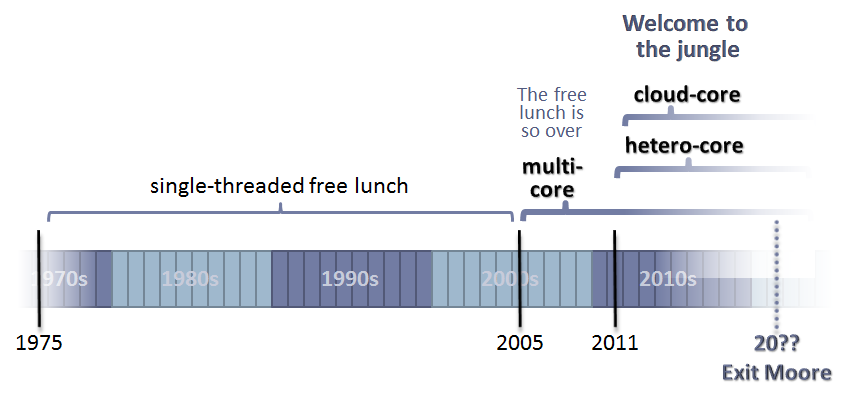
\includegraphics[width=0.9\textwidth]{img/free_lunsh.png}
\caption{Illustration of transitions between different eras in the computer industry. Currently there are three ongoing transitions; multi-core, heterogeneous-core and cloud-core. Image courtesy of Herb Sutter (herbsutter.com).}
\label{fig:jungle}
\end{figure}

Around the same time as CPU manufactures hit the frequency wall, people started experimenting with programmable shaders which recently had been introduced in the field of graphics programming. The graphics processing pipeline had before this been a fixed function pipeline, where e.g. geometry and textures where fed to the graphics processing unit (GPU) in one end and a rasterized rendered image was outputted in the other. What programmable shaders  introduced was the ability to replace some steps in the fixed-function pipeline with custom computations. This made it possible to utilize the GPU for other tasks than just rendering graphics \cite{Seland2007}. The rationale behind this exploration was that GPUs were already a highly available processor, and hidden behind its graphics interface was processing powers an order of magnitude larger than what the CPU could provide (Fig.\,\ref{fig:cpu_vs_gpu}). Actually, at the time when CPUs hit the frequency wall the GPU had already gone multi-core, driven by an ever-increasing demand for more realistic computer games. The rendering pipeline exhibits minimal execution path branching, and data are typically used once. Designers of GPUs could therefore skip advance feature, found in most CPUs, like branch prediction and different levels of data caching. This reduced the silicon footprint of each core and made it possible to add multiple cores to the same chip before CPU designers where able to do the same. Today, even if more advanced caching has been added to GPUs, this is still the main reason why GPUs have higher peak performance than CPUs (Fig.\,\ref{fig:cpu_vs_gpu}). Another reason is the inherent parallel nature of the rendering problem. When geometry is projected and rasterized the same instruction is typically needed for a lot of data at the same time. This makes a special kind of instruction, Single Instruction Multiple Data (\nom{SIMD}{Single instruction multiple data (instruction)}) instruction, especially suited for this kind of problem. The differences between how SIMD instructions are utilized in modern CPUs and GPUs is discussed in Section \ref{sec:cpu_vs_gpu}.

For the first adopters of GPU programming, or General-purpose programming on graphics processing units (GPGPU) as it was named, it soon became evident that offloading all types of computations to the GPU was not always a good idea. In most cases it is important to balance the load equally between the CPU and GPU to obtain their combined computationally power. Balancing typically means that highly parallel tasks should be offloaded to the GPU and serialized work should stay on the CPU. This paradigm of utilizing specialized cores for solving specific problems is today known as heterogeneous computing. The specialized core can 

FPGAs (Field-programmable gate array), APU (Accelerated processing unit).

Three currently ongoing transitions: Multi-core, Heterogeneous-cores, and Cloud-cores.

This thesis is focusing on heterogeneous computing with CPUs and GPUs. 

\subsection{Comparing CPU and GPU performance}\label{sec:cpu_vs_gpu}
It is common to say that a CPU has few but advance generic cores, and the GPU has many but simple cores.

It it is also much less costly to switch between a pixel-thread for the GPU then a program thread for the CPU.  

About theoretical FLOPS: Note that these are theoretical numbers and the actual throughput typically is algorithm dependent.

Compare CPU and GPU ALUs. SSE, AVX ... The GPU has super-wide registers. The SM in Fermi have 32 cores or 1024 bit registers. The SMX in Kepler have 192 cores. 6144 bit registers. SSE (Streaming SIMD Extensions) instructions have 128 bit registers. AVX (Advanced Vector Extensions) have 256 bit registers. AVX-512 has 512 bit registers. Single instruction, multiple data (SIMD).

\begin{figure}
\centering
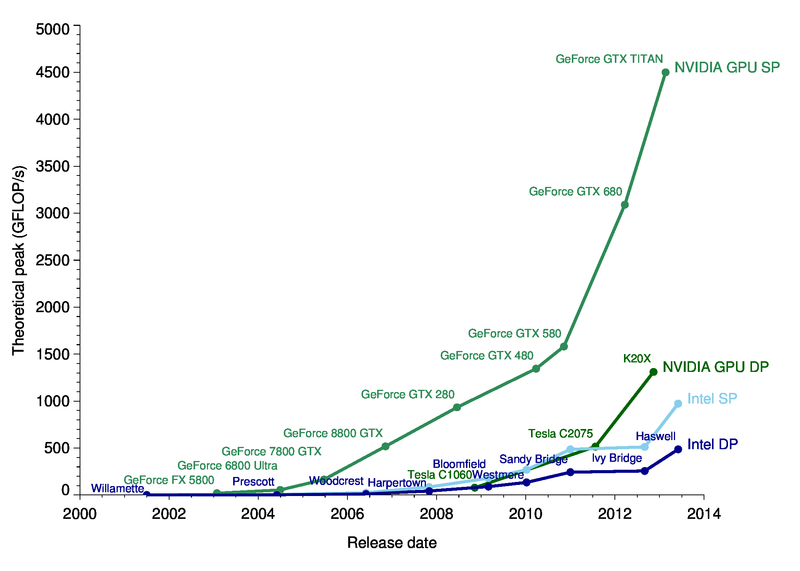
\includegraphics[width=0.9\textwidth]{img/cpu-vs-gpu.png}
\caption{Development in theoretical peak throughput, single precision (SP) and double precision (DP), the last decade for Intel CPUs and Nvidia GPUs. Image courtesy of Michael Galloy (michaelgalloy.com).}
\label{fig:cpu_vs_gpu}
\end{figure}

\subsection{Programming the GPU}
Early gpgpu programming required expert knowledge about graphics and the remaining fixed funtions in the pipeline. New programming languages where needed. OpenCL and CUDA. C++ AMP.

Architecture and how to program. See Paper II.

Hopefully, in the future, GPU programming will be the job of e.g. c++ compiler, and direct fiddling with GPU kernels should only be needed if maximum throughput is absolutely needed. (In the same way the compiler is able to translate c++ code into SSE and AVX instructions.)

\subsection{Accelerators in medical ultrasound imaging }
Add sentence about siemens and supersonic imagine scanners. They use GPUs? What does this mean? FPGAs and ASICs.

\begin{figure}
\centering
\subfigure[Threads, blocks and grid]{
	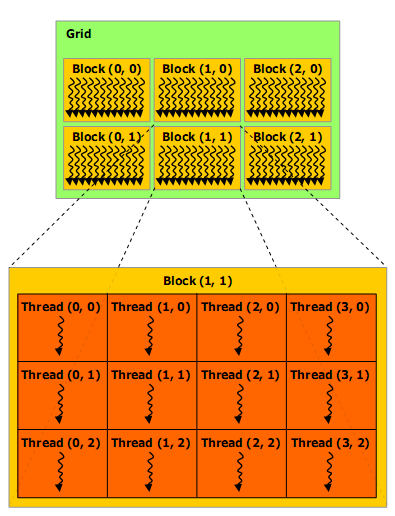
\includegraphics[width=0.4\textwidth]{img/cuda_threads.png}
}
\subfigure[Kernel]{
	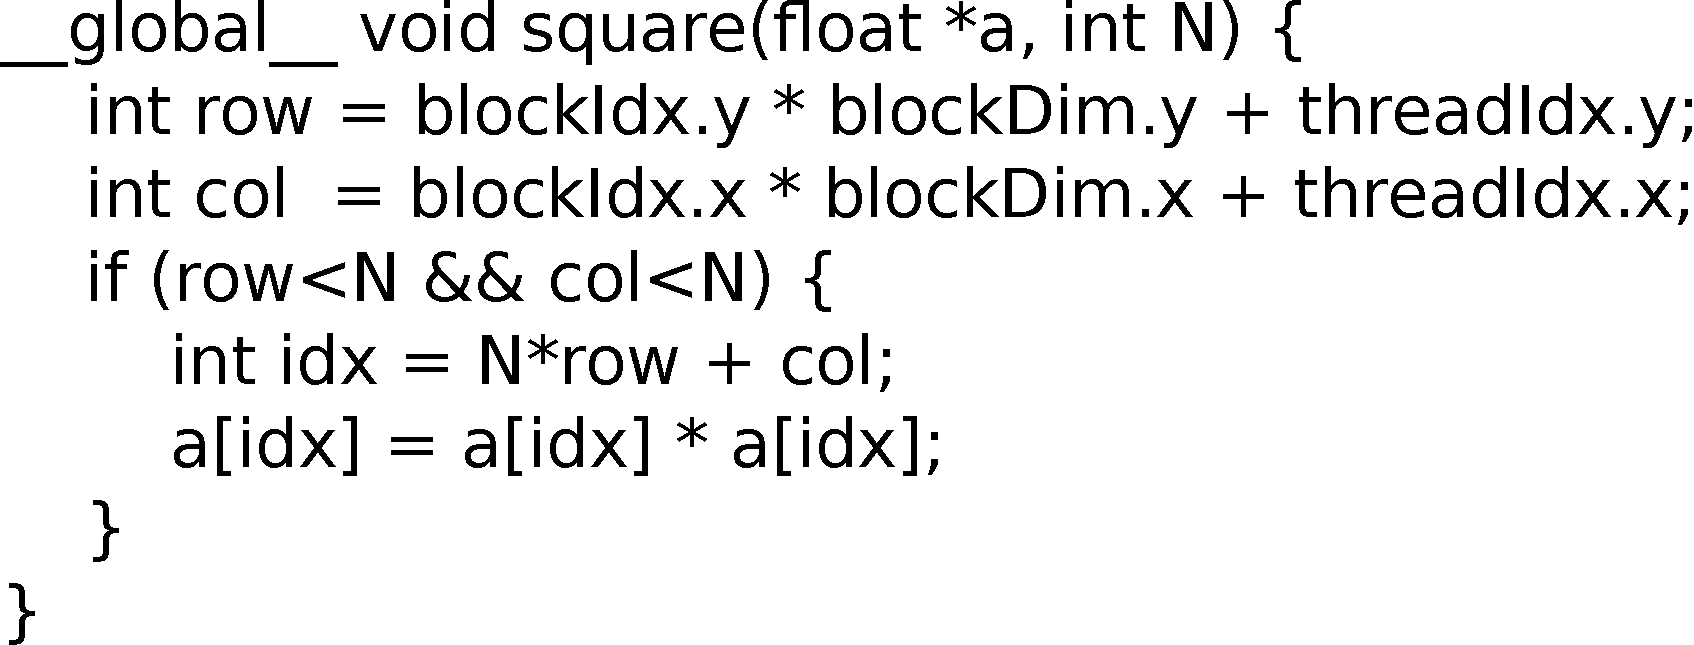
\includegraphics[width=0.5\textwidth]{img/kernel.pdf}
}
\caption{Depicts how GPU threads are grouped into blocks and arranged in a grid. One thread runs a copy of a kernel function, in this example an element-wise matrix square operation.}
\label{fig:gpu_grid}
\end{figure}

\section {Medical ultrasound imaging}\label{sec:ultrasound}
Ultrasound imaging encompasses technology which generates images based on sound whose frequencies we can not hear. For medical ultrasound imaging frequencies above 2 MHz are typically used.

Typical probes, scan sequences, resolution and sampling.

Key selling points of ultrasound imaging: cost, safety and real-time user interaction.

One sentence about speckle tracking.

\subsection{Cardiac anatomy}
Small section about heart anatomy.

\begin{figure}
\centering
\subfigure{
	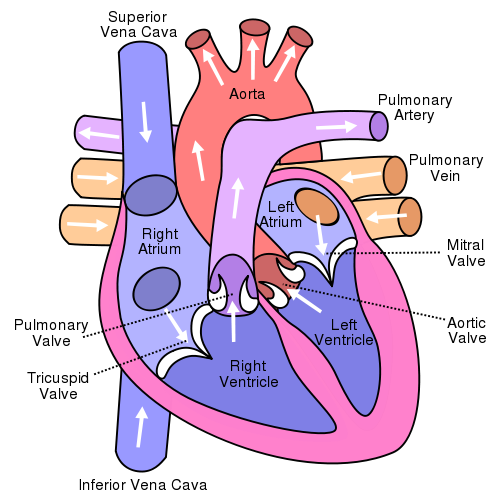
\includegraphics[width=0.47\textwidth]{img/Diagram_of_the_human_heart.png}
}
\subfigure{
	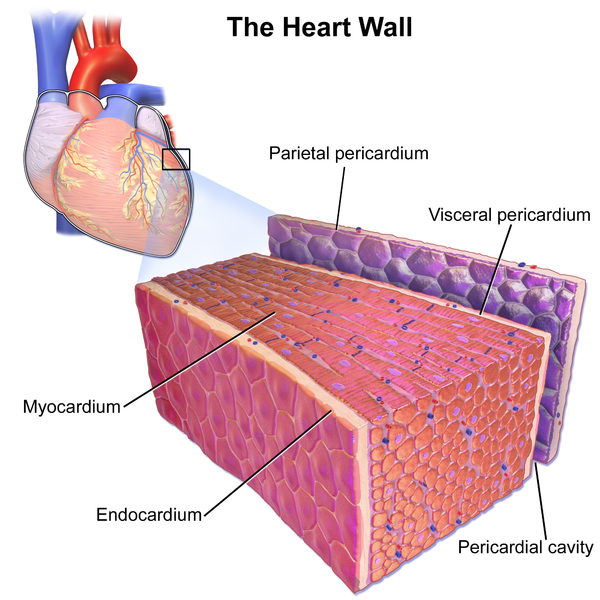
\includegraphics[width=0.47\textwidth]{img/HeartWall.png}
}
\caption{Overview of the human heart. Illustrations from wikipedia.org.}
\label{fig:human_heart}
\end{figure}
							
\subsection{Basic beamforming}

Delay and sum. Apodization. (See intro to Paper II or III).
Time v.s. phase delays.

\subsection{Adaptive Beamforming}\label{sec:adaptbf}

\begin{figure}[t!]
\subfigure[Delay-and-sum]{
	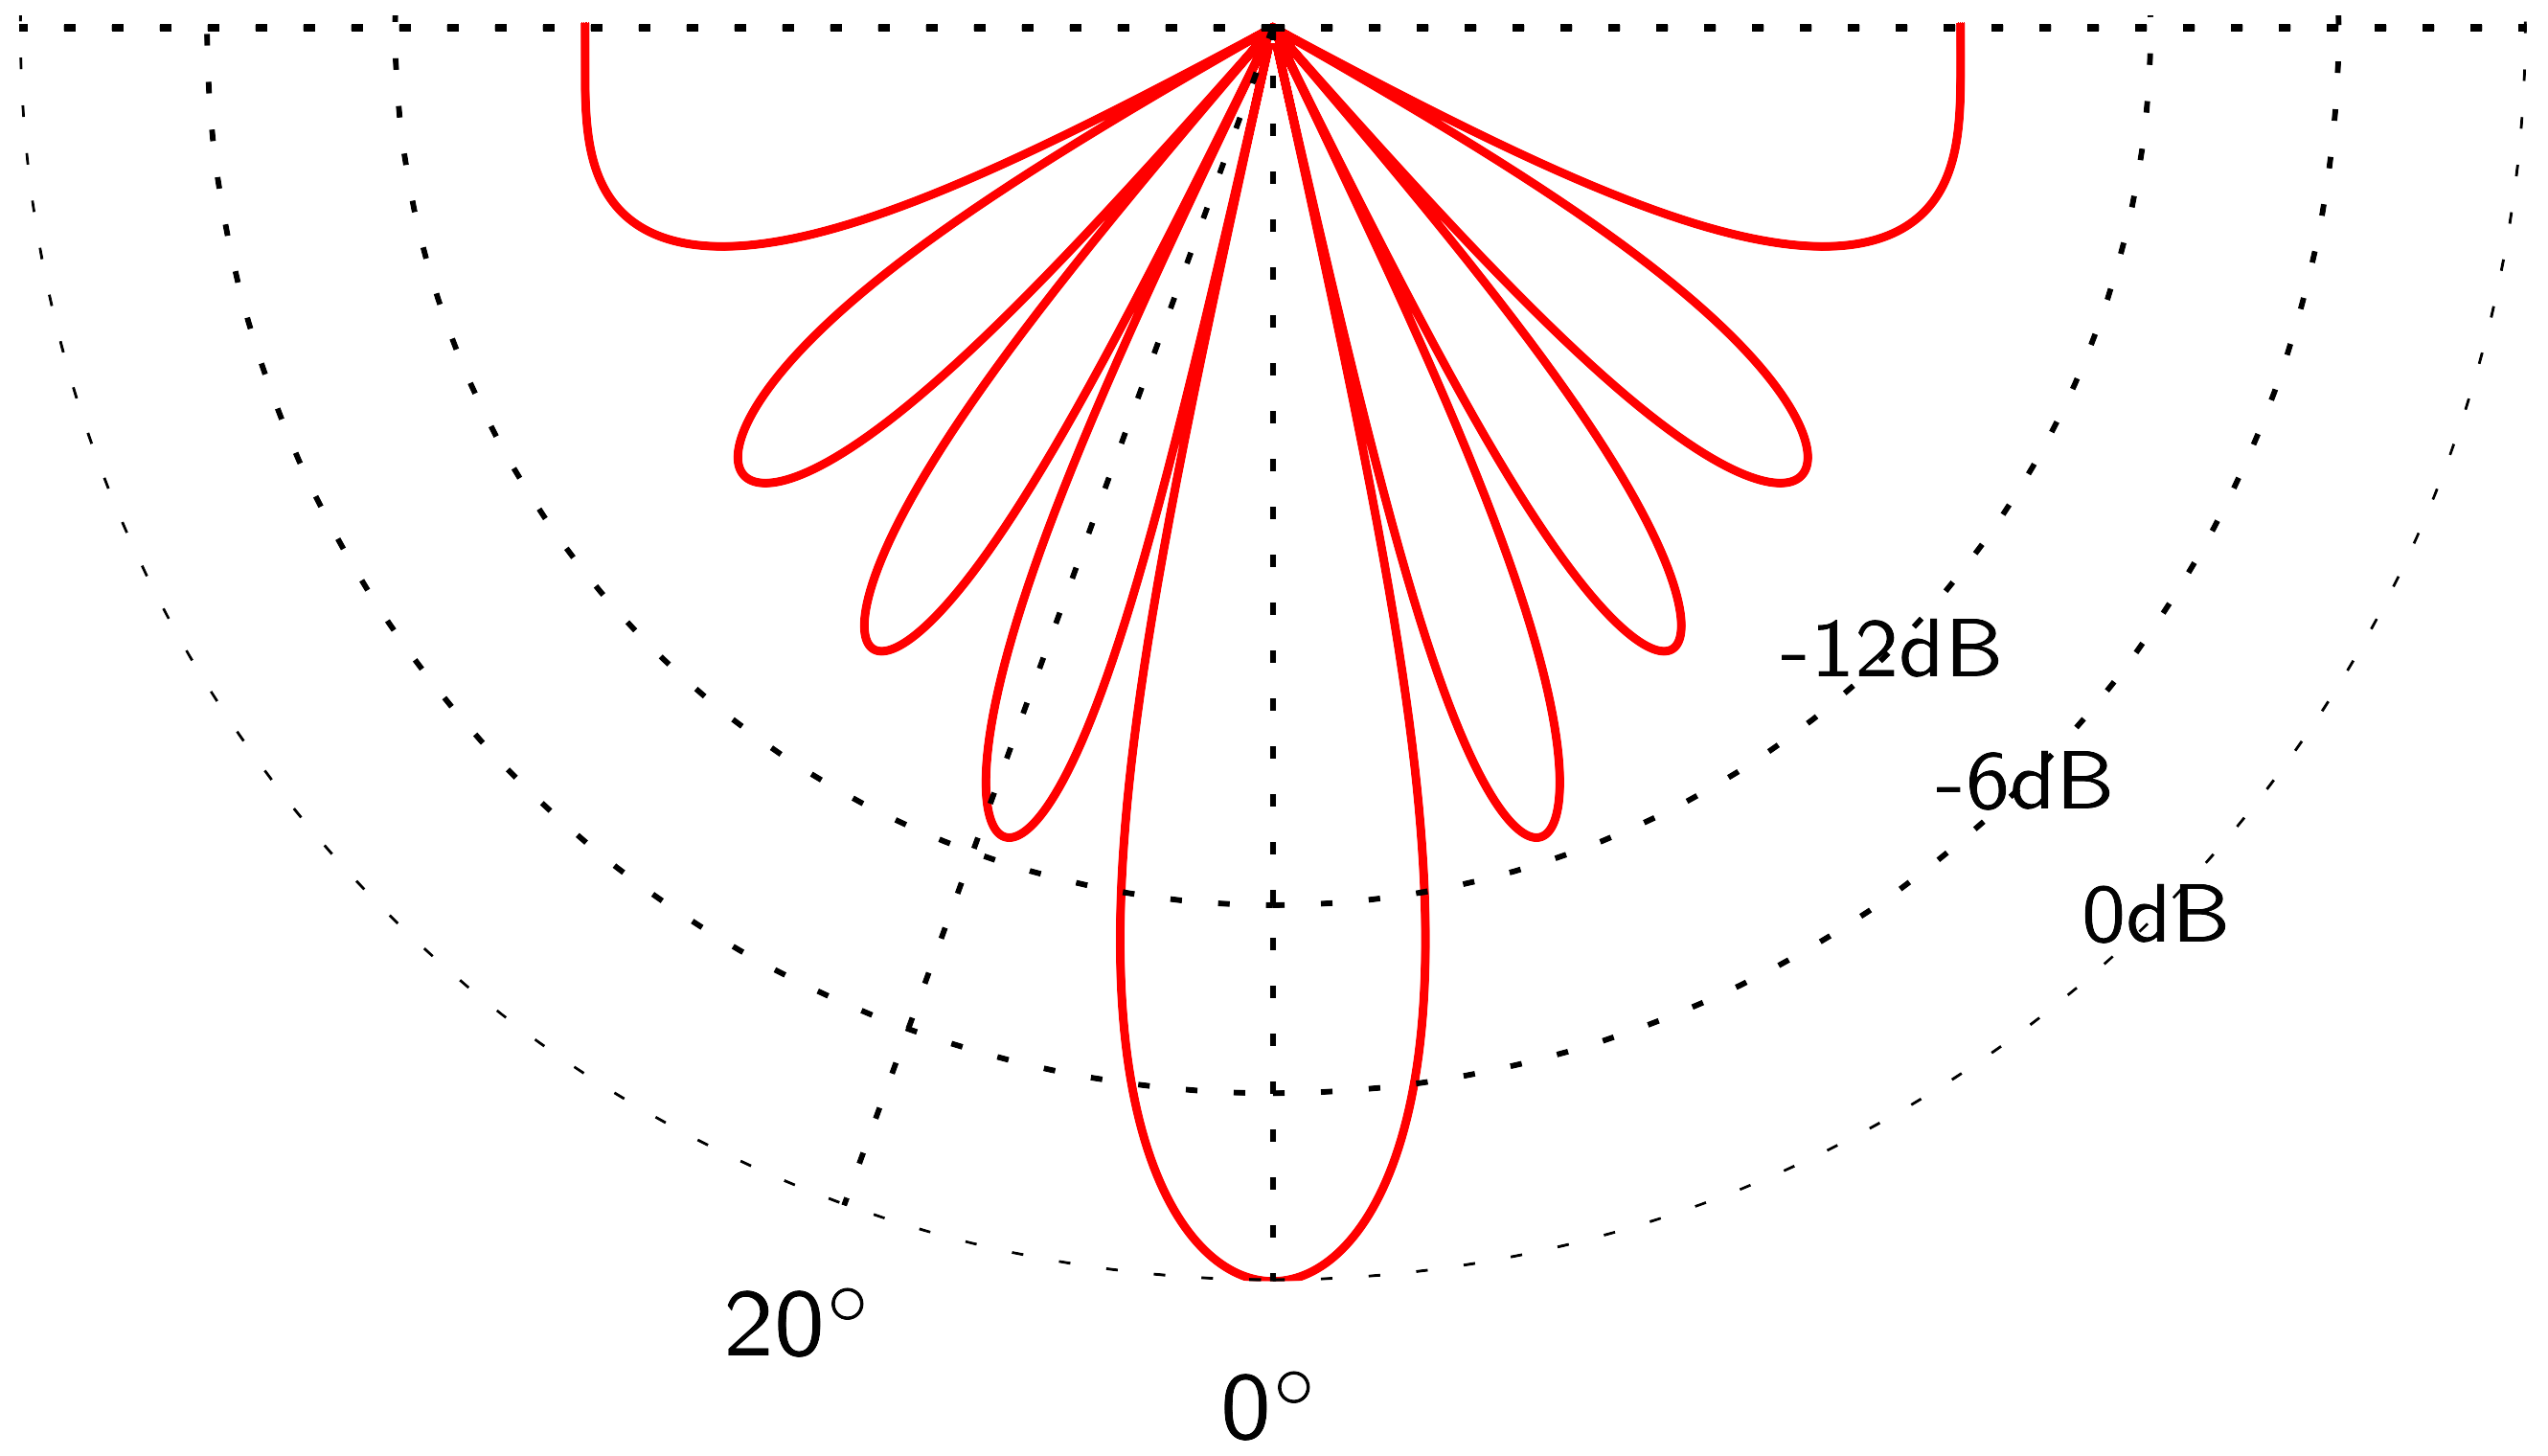
\includegraphics[width=0.47\textwidth]{img/scenario_das_resp2.png}
}
\subfigure[Capon]{
	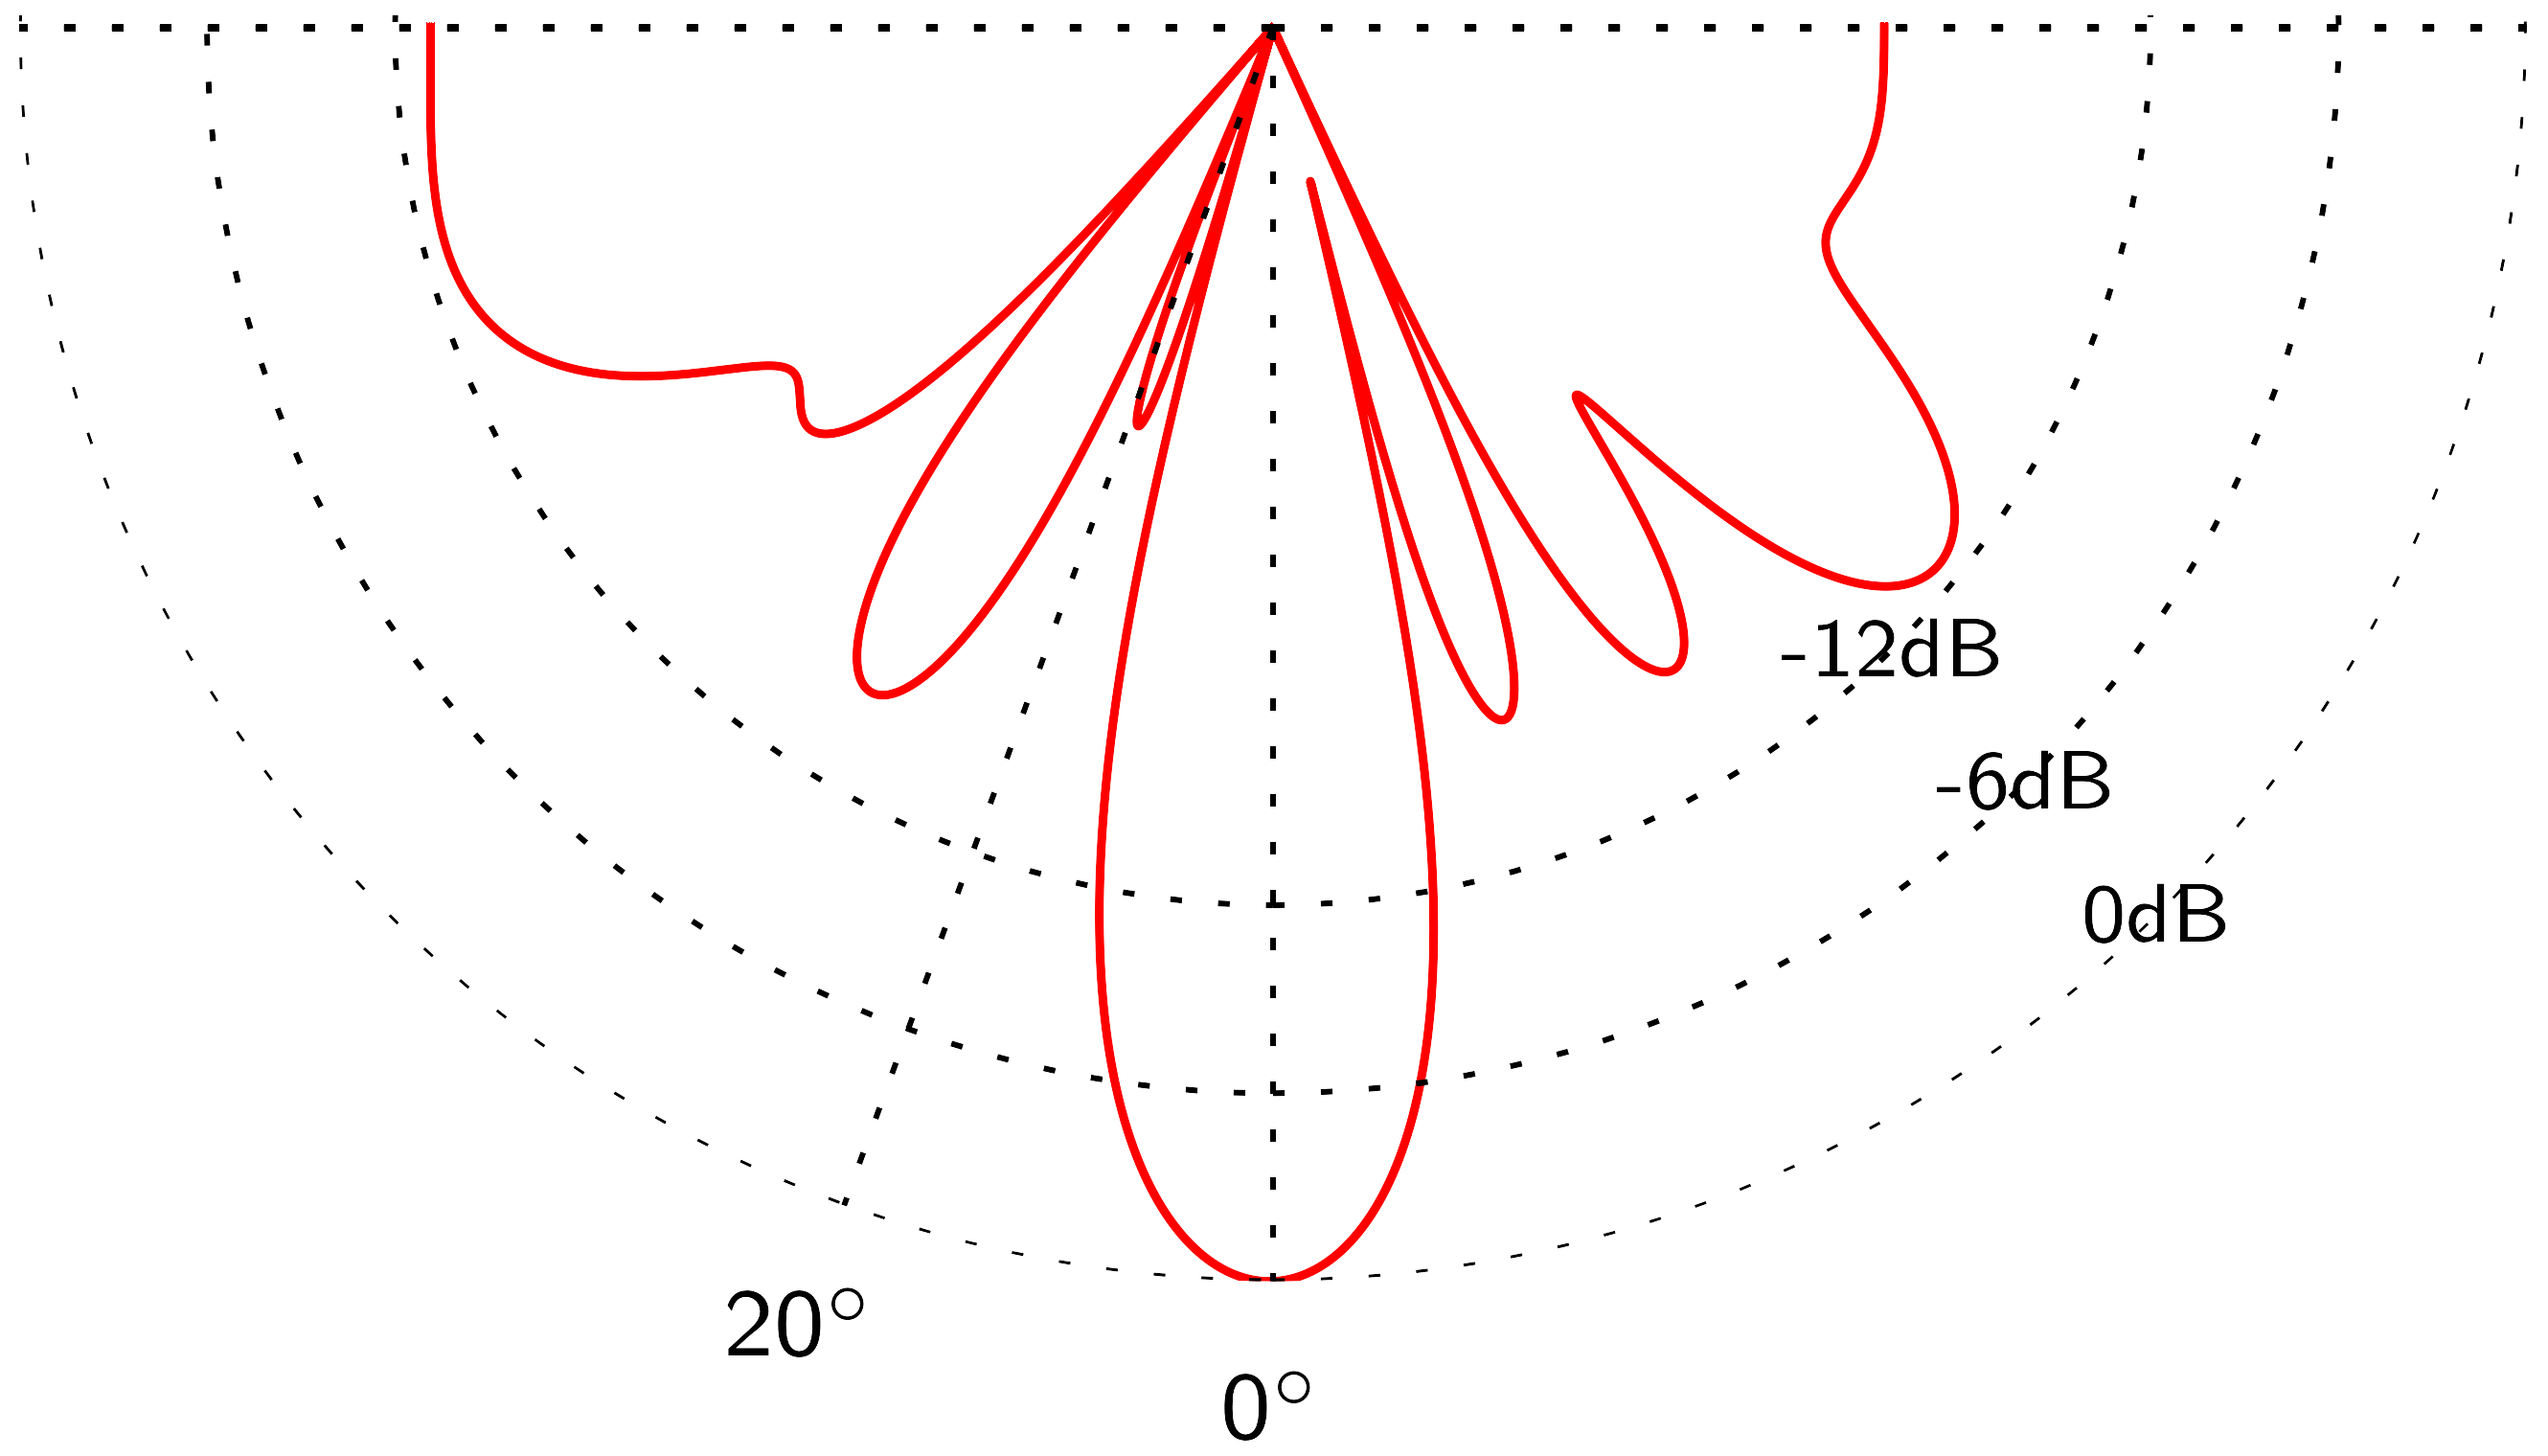
\includegraphics[width=0.47\textwidth]{img/scenario_mv_resp2.png}
}
\caption{Array beam pattern with uniform and Capon weights. An interfering source is located at 20 degrees.}
\end{figure}

Capon beamforming\footnote{The name ''Capon beamformer'' is due to work by J. Capon \todo{add citation} on seismic arrays \todo{Move to background.}} or minimum variance beamforming.

Intro to adaptive beamforming. List other variants (LCA, beamspace, Eigen space etc.). 

Beamspace data is typically refers to the polar grid that cardiac ultrasound data is located in prior to scan conversion. In combination with the Capon beamformer, beamspace refers to the K-space representation of the impinging signals (hence the \nom{FFT}{Fast fourier transform} of the channel data). 

Not phase aberration correction.

Add section about the computationally complexity. How many flops are required per rx-beam etc...

Add section about how to present data (max v.s mean etc.)
						
\subsection{Shift invariance}

\section{Volume rendering}\label{sec:volren}

Get section from master theses. Ray casting and opacity functions.

\begin{figure}
\centering
\subfigure[Ray-casting]{
	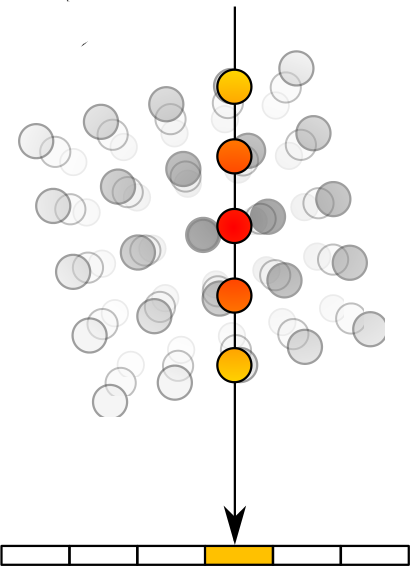
\includegraphics[width=0.4\textwidth]{img/Volumeraycasting.png}
}
\subfigure[Opacity transfer function]{
	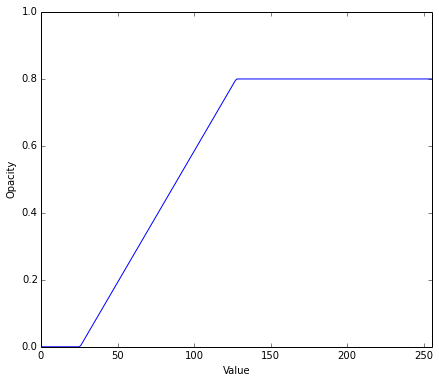
\includegraphics[width=0.5\textwidth]{img/otf.png}
}
\caption{.}
\label{fig:vr}
\end{figure}

\subsection{Adaptive volume rendering}

Visibility driven visualization.

\section{Field simulations}\label{sec:field}

Small chapter about different simulation tools (See hos paper).
			
\endinput
